\section{\texorpdfstring{\reviewchange{Masked Diffusion}}{Masked Diffusion}}
\label{app:absorbing process}

\begin{reviewblock}
This appendix expands the masked diffusion process used by MDLM. The section
has two parts. First, in Appendix~\ref{app:mdlm-formulation-theory}, we
describe the MDLM forward process, training objective, and reverse sampler.
Second, in Appendix~\ref{app:mdlm-inverse-distillation}, we explain why this
process gives a particularly simple inverse distillation signal. Masked
diffusion is a process-specific instance of the general continuous-time Markov
chain (CTMC) formulation in
Appendix~\ref{app:details of considered processes}, where ordinary tokens move
to the mask state.

\subsection{\texorpdfstring{Masked Diffusion Formulation and Theory}{Masked Diffusion Formulation and Theory}}
\label{app:mdlm-formulation-theory}

Masked diffusion corrupts text by replacing clean tokens with a special mask
token. Reverse sampling then gradually reveals the masked positions. This
process is also called absorbing diffusion because, once a token reaches the
mask state in the forward process, it stays there.

\paragraph{Forward process.}
Let $m\in\VC$ be the mask token. We use column-vector
conventions throughout: probability vectors are columns, and each diffusion
matrix has columns that sum to zero. The absorbing process sends every
non-mask token to $m$ and leaves $m$ fixed. Hence its terminal distribution is
the point mass $\pi=m$.

The base generator of this continuous-time Markov chain is
\begin{equation}
    Q_{\text{abs}} =
    \begin{bmatrix}
        -1 & 0 & \cdots & 0 & 0 \\
        0 & -1 & \cdots & 0 & 0 \\
        \vdots & \vdots & \ddots & \vdots & \vdots \\
        0 & 0 & \cdots & -1 & 0 \\
        1 & 1 & \cdots & 1 & 0
    \end{bmatrix}.
\end{equation}
With time-dependent rate $\sigma_t$, the forward generator is
\begin{equation}
    \label{eq: absorbing diffusion matrix}
    Q_t = \sigma_t Q_{\text{abs}} =
    \begin{bmatrix}
        -\sigma_t & 0 & \cdots & 0 & 0 \\
        0 & -\sigma_t & \cdots & 0 & 0 \\
        \vdots & \vdots & \ddots & \vdots & \vdots \\
        0 & 0 & \cdots & -\sigma_t & 0 \\
        \sigma_t & \sigma_t & \cdots & \sigma_t & 0
    \end{bmatrix}.
\end{equation}
If $\bar{\sigma}_t\vcentcolon=\int_0^t\sigma_sds$, then the cumulative
transition matrix is
\begin{equation}
    \exp(\bar{\sigma}_t Q_{\text{abs}}) =
    \begin{bmatrix}
        \exp(-\bar{\sigma}_t) & 0 & \cdots & 0 & 0 \\
        0 & \exp(-\bar{\sigma}_t) & \cdots & 0 & 0 \\
        \vdots & \vdots & \ddots & \vdots & \vdots \\
        0 & 0 & \cdots & \exp(-\bar{\sigma}_t) & 0 \\
        1 - \exp(-\bar{\sigma}_t) & 1 - \exp(-\bar{\sigma}_t) & \cdots & 1 - \exp(-\bar{\sigma}_t) & 1
    \end{bmatrix}.
\end{equation}
Equivalently, with $\alpha_t\vcentcolon=\exp(-\bar{\sigma}_t)$, a clean token
$x_0$ is preserved with probability $\alpha_t$ and absorbed into the mask with
probability $1-\alpha_t$:
\[
    q_t(x_t\mid x_0)
    =
    \mathrm{Cat}\bigl(x_t;\alpha_t x_0 + (1-\alpha_t)m\bigr).
\]
Thus, at any time $t$, a token has only two possible forward states: it is
still equal to the original clean token, or it has become the mask token.
Figure~\ref{fig:masked-forward-kernel} shows the same kernel visually. The
important point is that the masked kernel is linear in the clean-token
distribution: it can be applied either to a hard one-hot token or to the
simplex-valued generator output used later in IDLM.

\begin{figure*}[t]
    \centering
    \begin{subfigure}[b]{0.48\textwidth}
        \centering
        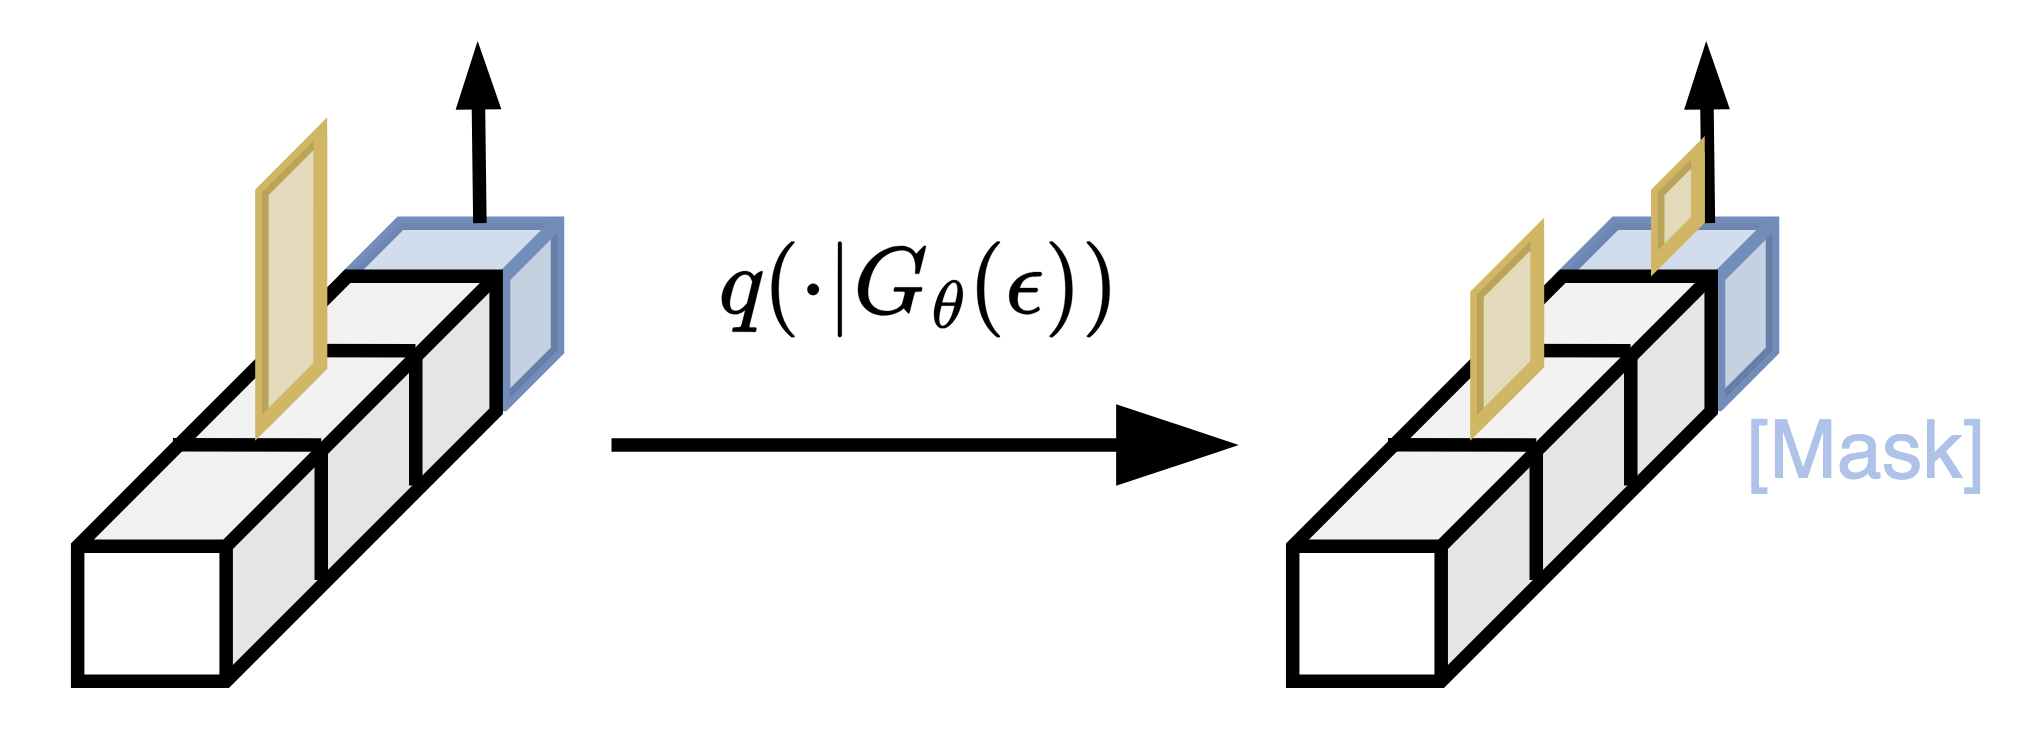
\includegraphics[width=\linewidth]{images/appendix_b_forward_onehot.png}
        \caption{Hard one-hot input.}
    \end{subfigure}
    \hfill
    \begin{subfigure}[b]{0.48\textwidth}
        \centering
        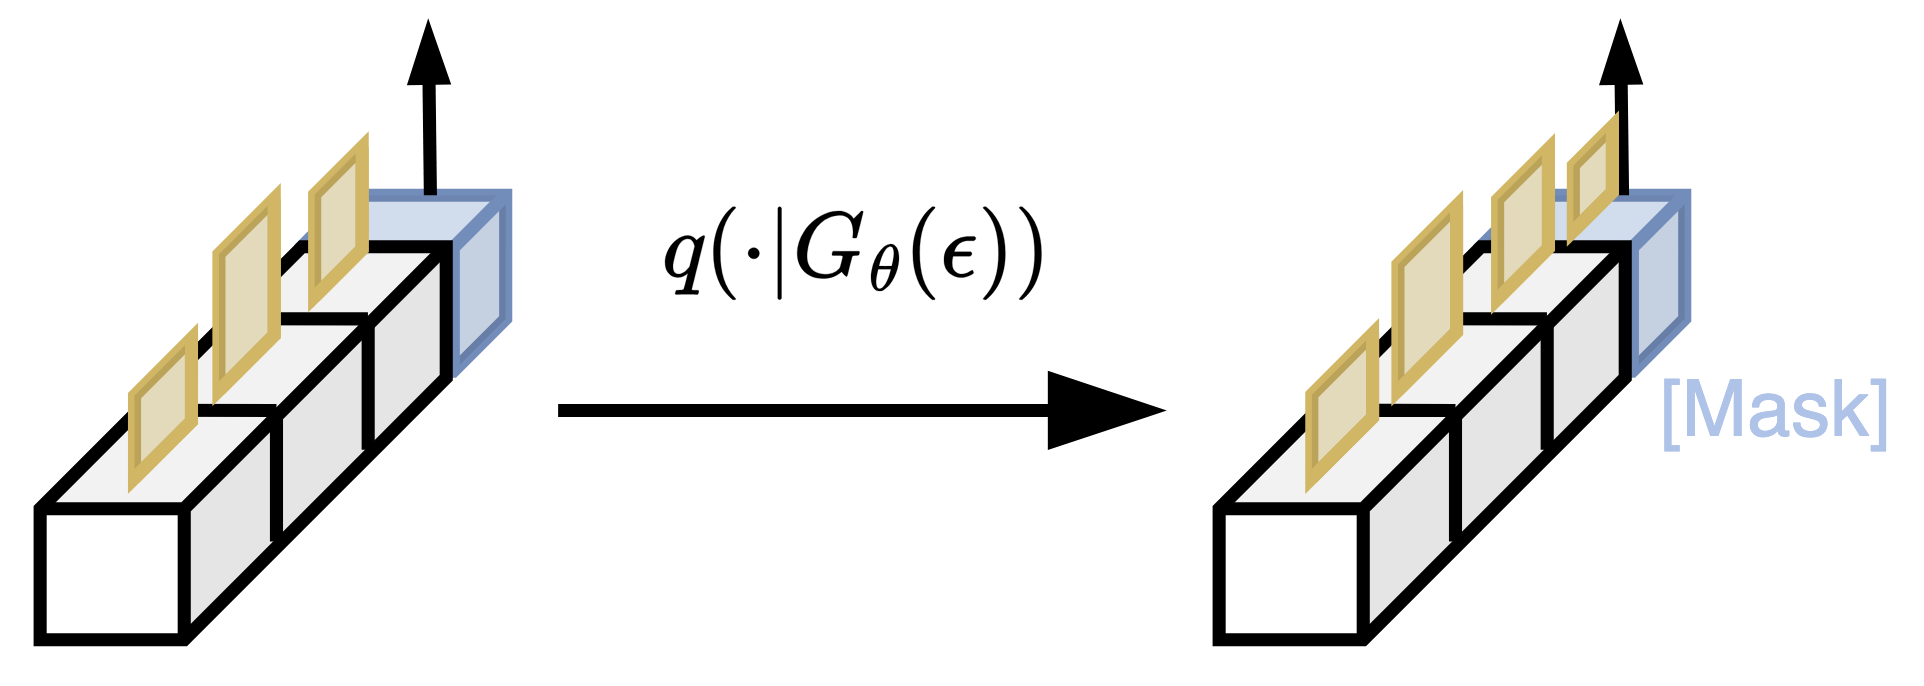
\includegraphics[width=\linewidth]{images/appendix_b_forward_simplex.png}
        \caption{Simplex-valued input.}
    \end{subfigure}
    \caption{Masked forward process. The transition
    $q_t(\cdot\mid x_0)$ preserves the clean-token mass with probability
    $\alpha_t$ and moves the remaining mass to the mask token. Because this map
    is linear, the same operation applies to a one-hot token and to a
    differentiable simplex output $G_\theta(\epsilon)$.}
    \label{fig:masked-forward-kernel}
\end{figure*}

\paragraph{Training loss.}
MDLM~\citep{sahoo2024simple, shi2024simplified} uses this absorbing process
with a clean-token predictor $f(x_t,t)\in\Delta$. Training is weighted
masked-token prediction: when a position has been absorbed into the mask, the
model predicts its original clean token.

\paragraph{Sampling procedure.}
Sampling starts from the terminal distribution, i.e. from a fully masked
sequence, and then integrates the learned reverse process toward $t=0$.
For $0\leq s<t\leq1$, let $f_t\vcentcolon=f(x_t,t)$. MDLM uses the absorbing
posterior with the true clean token replaced by the model prediction:
\[
\begin{aligned}
p^{f}_{s\mid t}(x_s\mid x_t)
&=
\begin{cases}
    \mathrm{Cat}(x_s; x_t), & x_t\neq m,\\[2pt]
    \mathrm{Cat}\!\left(x_s;\dfrac{1-\alpha_s}{1-\alpha_t}m
    + \dfrac{\alpha_s-\alpha_t}{1-\alpha_t}f_t\right), & x_t=m .
\end{cases}
\end{aligned}
\]
Figure~\ref{fig:masked-diffusion-sampling-intuition} visualizes this reverse
sampling path. The two cases simply say that masked diffusion is one-way: a
revealed token stays revealed, while a masked token can either stay masked or be
revealed. This is the \textsc{subs} sampling rule used by MDLM. If the token has
already been revealed, \textsc{subs} copies it unchanged. If the token is still
masked, the reverse step either keeps it masked until time $s$ or reveals it
according to the clean-token prediction $f_t$. The noise schedule controls how
many tokens are still masked at each time. The model controls which token is
chosen when a masked position is revealed.

\begin{figure*}[t]
    \centering
    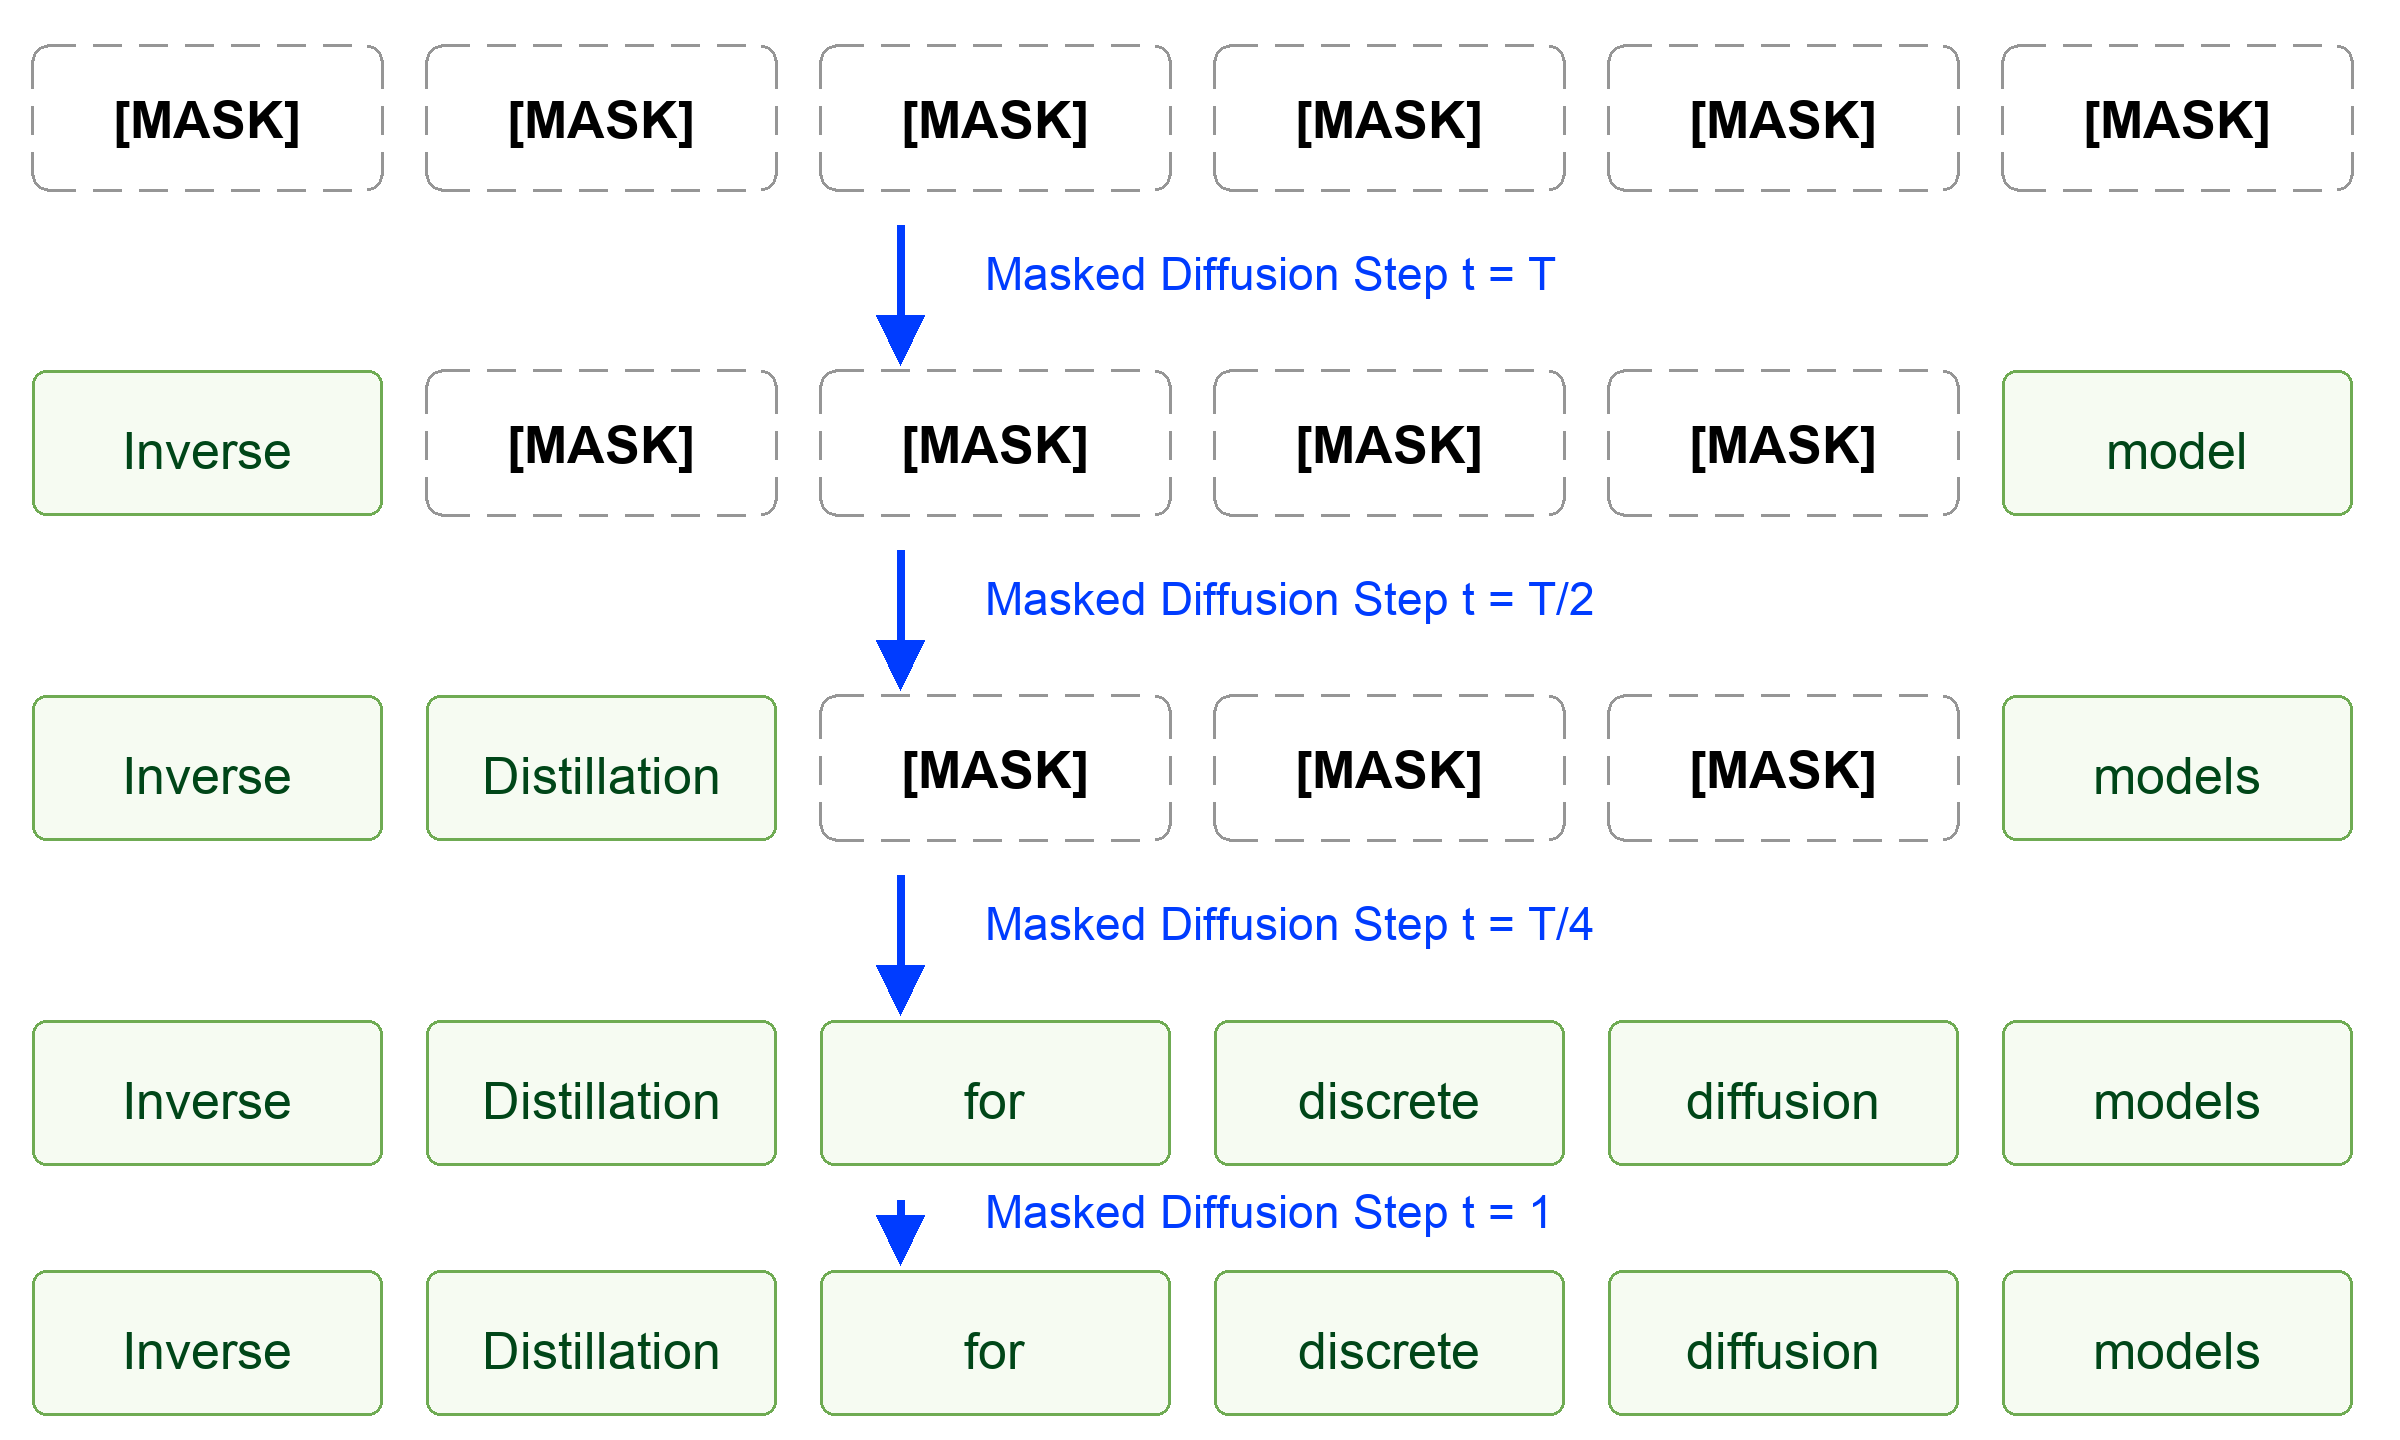
\includegraphics[width=0.95\textwidth]{images/masked_diffusion_sampling_standalone.png}
    \caption{Masked-diffusion sampling procedure. The sampler
    starts from a
    fully masked sequence and reveals each position once; after a token is
    revealed, later reverse steps copy it. Thus the schedule decides when a
    position is revealed, and the model decides which token to put there.}
    \label{fig:masked-diffusion-sampling-intuition}
\end{figure*}

This is the main contrast with uniform diffusion. In masked diffusion, revealed
tokens stay fixed. In uniform diffusion, tokens can still change later, so the
IDLM signal for uniform diffusion must track intermediate states; see
Appendix~\ref{app:uniform process} for the corresponding uniform-diffusion
formulation.

\subsection{\texorpdfstring{Inverse Distillation for Masked Diffusion}{Inverse Distillation for Masked Diffusion}}
\label{app:mdlm-inverse-distillation}

We now connect the masked diffusion process to the IDLM objective. The general
inverse distillation loss, introduced in
Section~\ref{sec:inverse distillation}, asks for a student distribution
$p_\theta$ on which the pretrained teacher $f^*$ is better than any diffusion
model trained only on student samples:
\[
    \LC_{\mathrm{IDLM}}(\theta)
    =
    \LC(f^*,p_\theta)-\min_{\tilde f}\LC(\tilde f,p_\theta).
\]
In practice, the inner minimizer is represented by a fake model $f$ trained
on the current student distribution, as in the alternating optimization in
Section~\ref{sec:loss intuition}. Therefore, during a generator step we use the
teacher-minus-fake objective
\[
    \LC_{\mathrm{IDLM}}(\theta)
    =
    \LC(f^*,p_\theta)-\LC(f,p_\theta).
\]
For masked diffusion, this gap has an especially transparent form because of
the \textsc{subs} parameterization.

\paragraph{Simplex relaxation.}
The student generator should ultimately choose vocabulary tokens, but a hard
one-hot output blocks ordinary backpropagation. We therefore allow the
generator output to lie in the simplex, following
Section~\ref{sec:simplex relaxation},
\[
    G_\theta(\epsilon)\in\Delta .
\]
This is still a valid token distribution: its entries are nonnegative and sum
to one. Moreover, the masked forward kernel remains well-defined, as illustrated
in Figure~\ref{fig:masked-forward-kernel}, because
\[
    \alpha_t G_\theta(\epsilon)+(1-\alpha_t)m\in\Delta .
\]
Thus the generator update can use a weighted sum over possible clean tokens
instead of committing to one sampled token before gradients are computed.
Figure~\ref{fig:mdlm-simplex-relaxation} shows the relaxation: the discrete
target is a one-hot token, but during optimization the generator can expose
continuous token weights.

\begin{figure*}[t]
    \centering
    \begin{subfigure}[b]{0.18\textwidth}
        \centering
        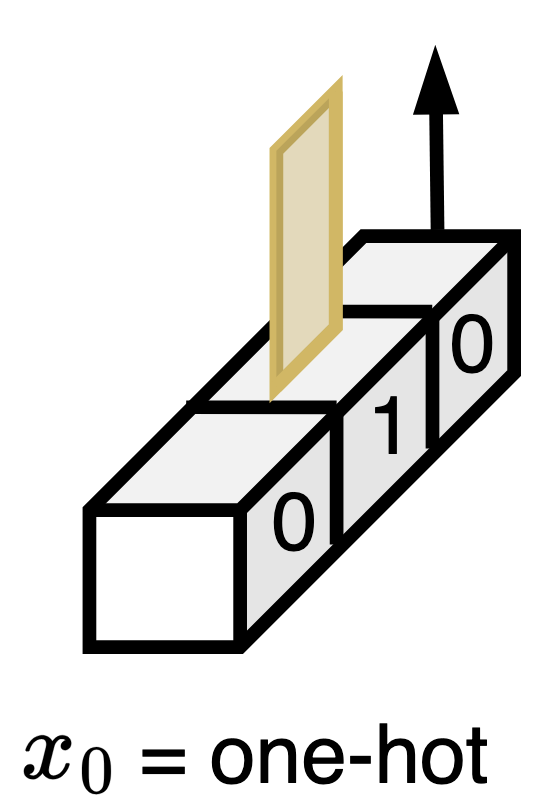
\includegraphics[width=\linewidth]{images/appendix_b_onehot_token.png}
        \caption{Discrete token.}
    \end{subfigure}
    \hfill
    \begin{subfigure}[b]{0.39\textwidth}
        \centering
        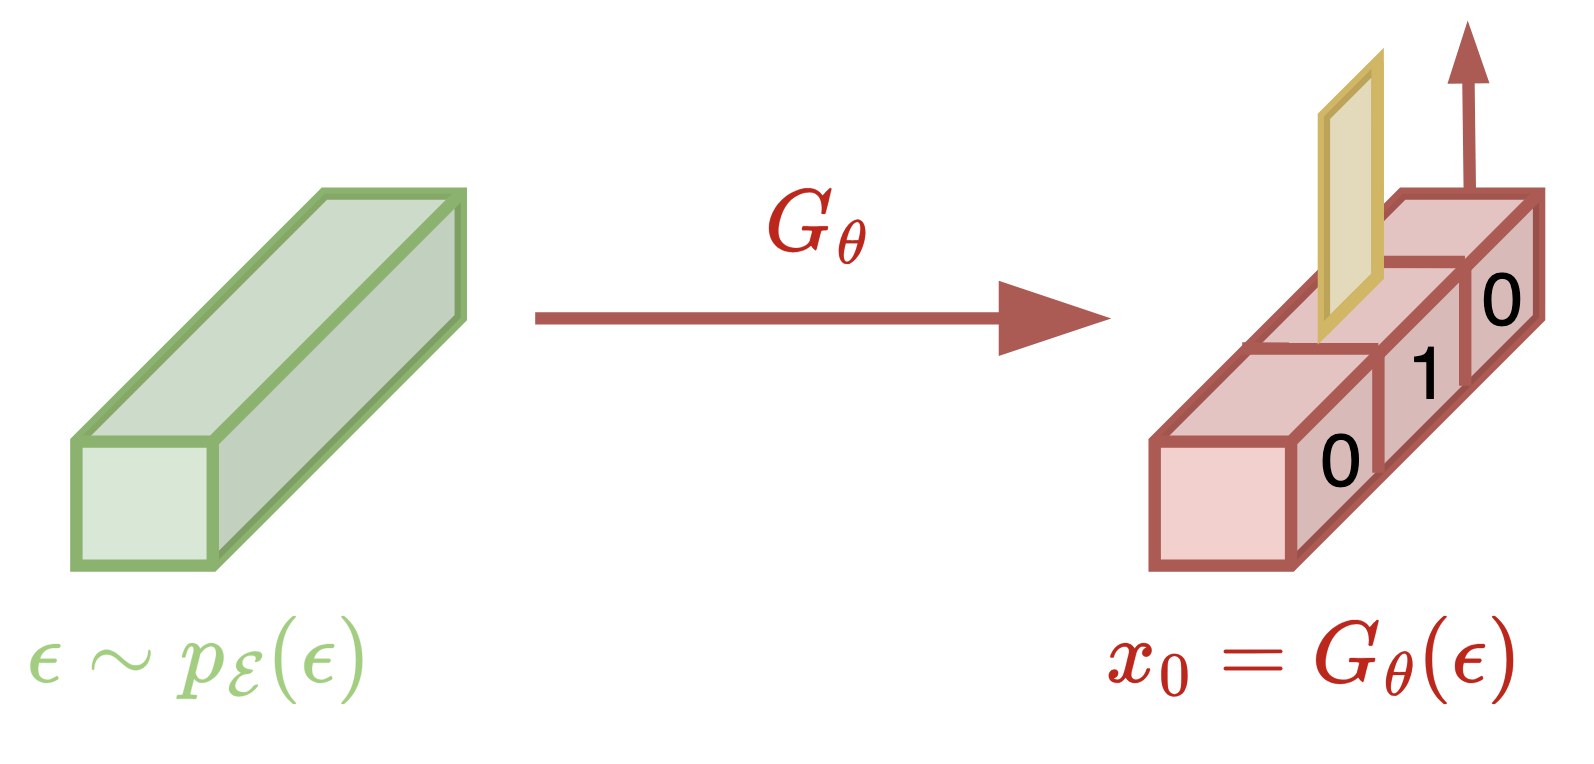
\includegraphics[width=\linewidth]{images/appendix_b_generator_onehot.png}
        \caption{Hard generator output.}
    \end{subfigure}
    \hfill
    \begin{subfigure}[b]{0.39\textwidth}
        \centering
        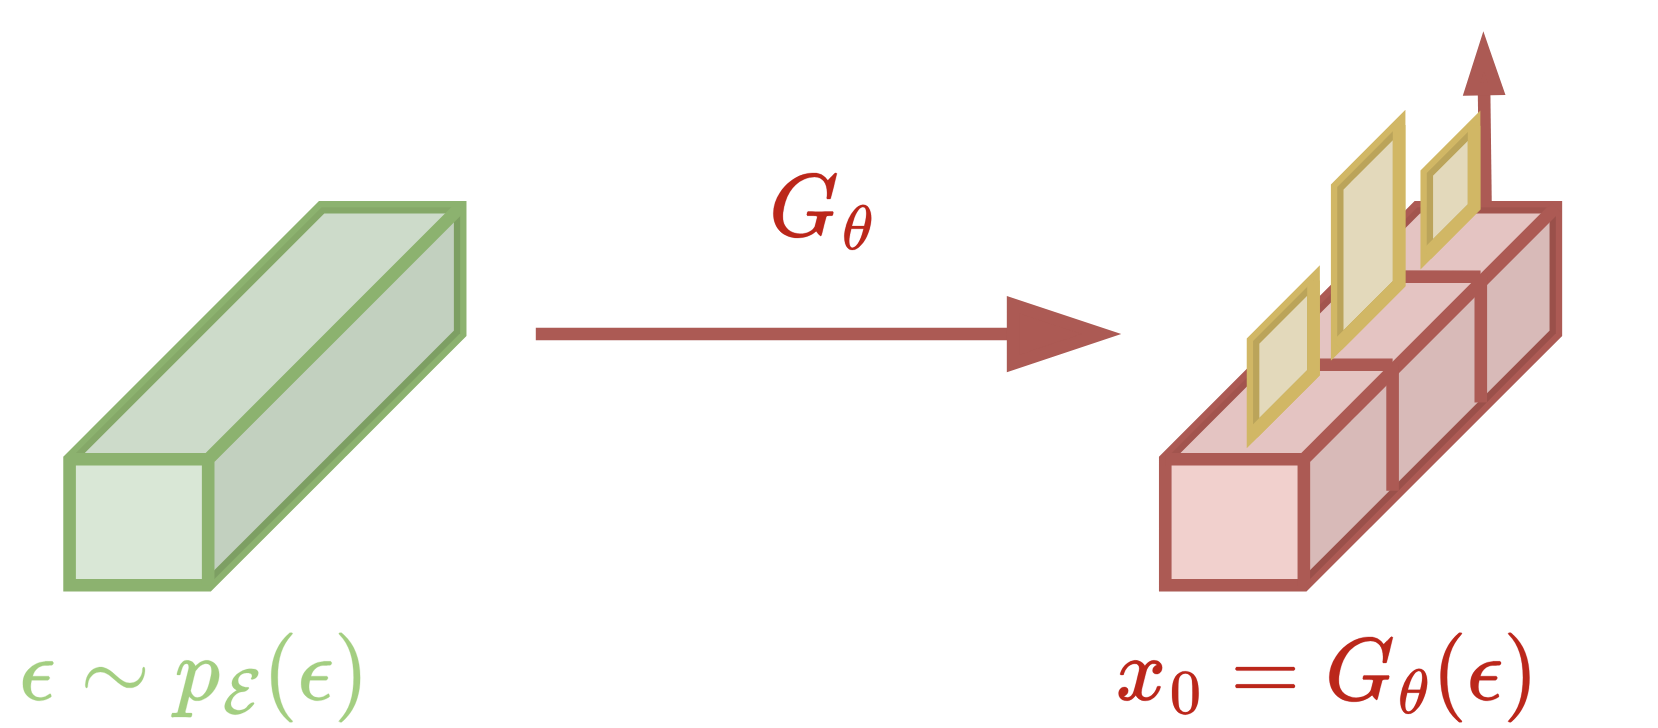
\includegraphics[width=\linewidth]{images/appendix_b_generator_simplex.png}
        \caption{Simplex generator output.}
    \end{subfigure}
    \caption{Simplex relaxation for IDLM-MDLM, following
    Section~\ref{sec:simplex relaxation}. A generated token is ultimately
    interpreted as a one-hot vocabulary choice, but the generator update uses
    $G_\theta(\epsilon)\in\Delta$ so gradients can weight several candidate
    tokens before a hard sample is chosen.}
    \label{fig:mdlm-simplex-relaxation}
\end{figure*}

This also changes how the token loss should be read. With a hard one-hot
target, the inner product with $\log f(x_t,t)$ simply picks the log-probability
of one token. With $G_\theta(\epsilon)\in\Delta$, the same inner product becomes
a weighted sum over token log-probabilities, as shown in
Figure~\ref{fig:mdlm-token-loss}.

\begin{figure*}[t]
    \centering
    \begin{subfigure}[b]{0.48\textwidth}
        \centering
        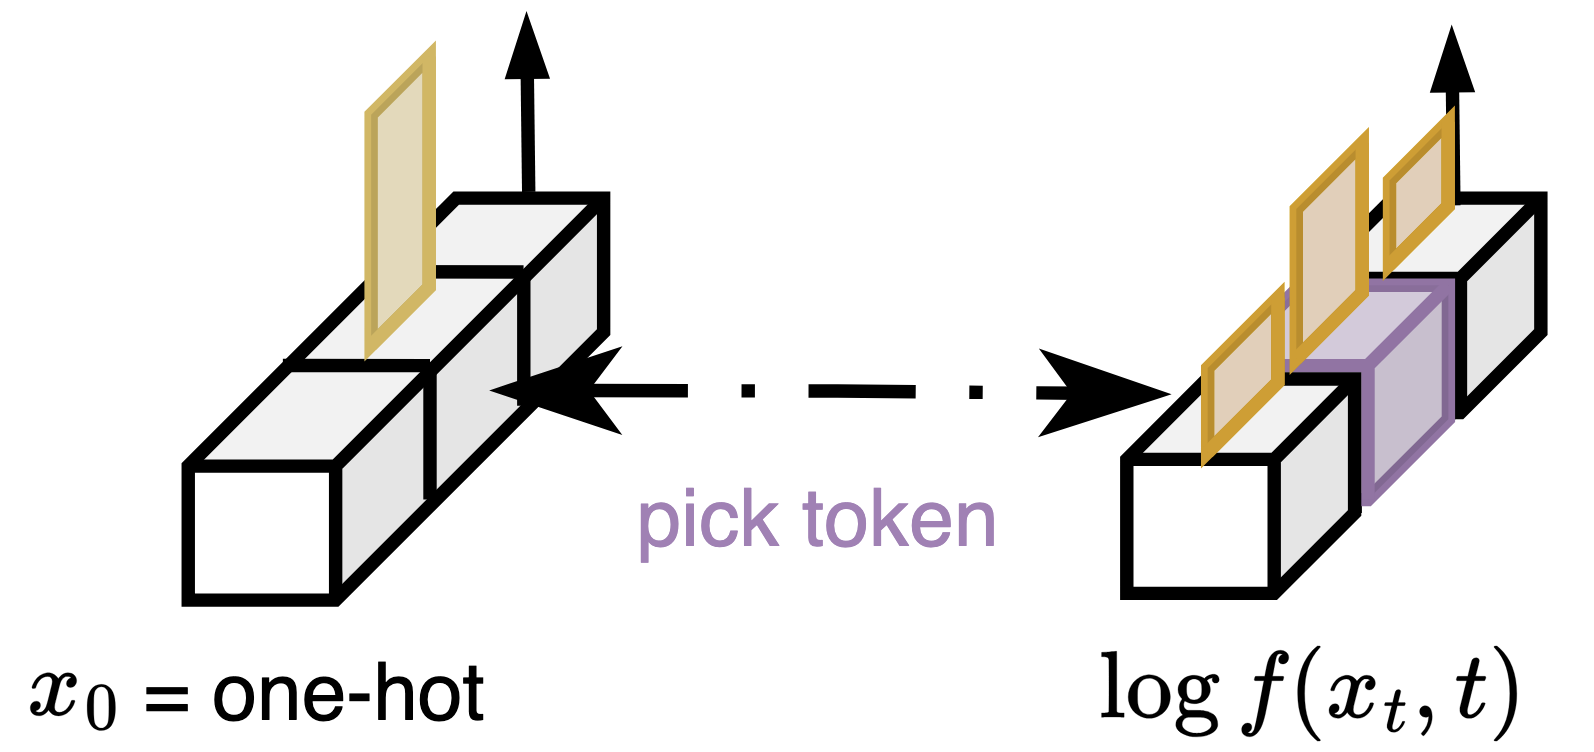
\includegraphics[width=\linewidth]{images/appendix_b_pick_token_loss.png}
        \caption{One-hot target: pick one coordinate.}
    \end{subfigure}
    \hfill
    \begin{subfigure}[b]{0.48\textwidth}
        \centering
        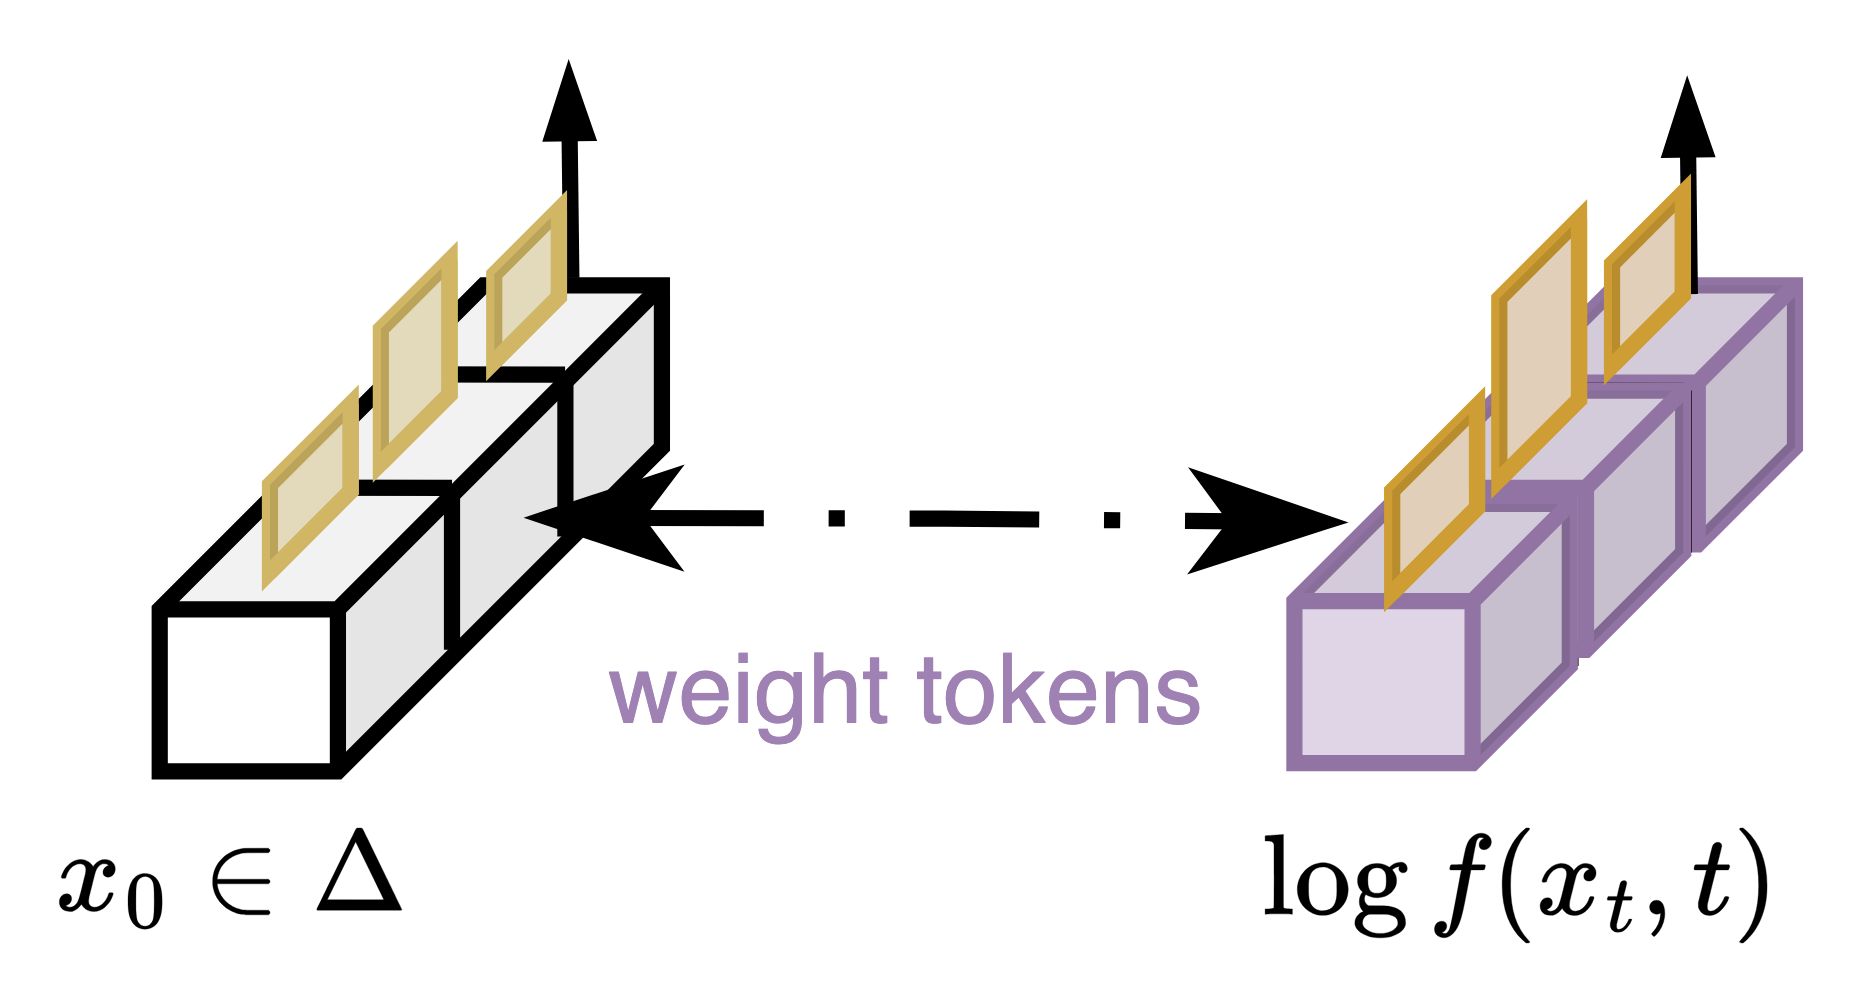
\includegraphics[width=\linewidth]{images/appendix_b_weight_tokens_loss.png}
        \caption{Simplex target: weight token coordinates.}
    \end{subfigure}
    \caption{Loss evaluation under the simplex relaxation.
    The one-hot case selects a single log-probability from $\log f(x_t,t)$,
    while the simplex case evaluates the weighted sum
    $\langle G_\theta(\epsilon),\log f(x_t,t)\rangle$.}
    \label{fig:mdlm-token-loss}
\end{figure*}

\paragraph{Mask-only cancellation.}
The \textsc{subs} parameterization copies any already unmasked token:
\[
    x_t\neq m
    \quad\Longrightarrow\quad
    f^*(x_t,t)=f(x_t,t)=x_t .
\]
Therefore, for non-mask states, the teacher and fake model make the same
prediction and their contributions cancel in the IDLM gap. Only masked states
remain. Figure~\ref{fig:mdlm-subs-cancellation} gives the presentation view of
this cancellation. If the forward process returns an unmasked state, the state
is already the clean token, so both the teacher and the fake model copy it. If
the forward process returns the mask state, the model must infer the clean
token, and this is where the IDLM signal survives.

\begin{figure*}[t]
    \centering
    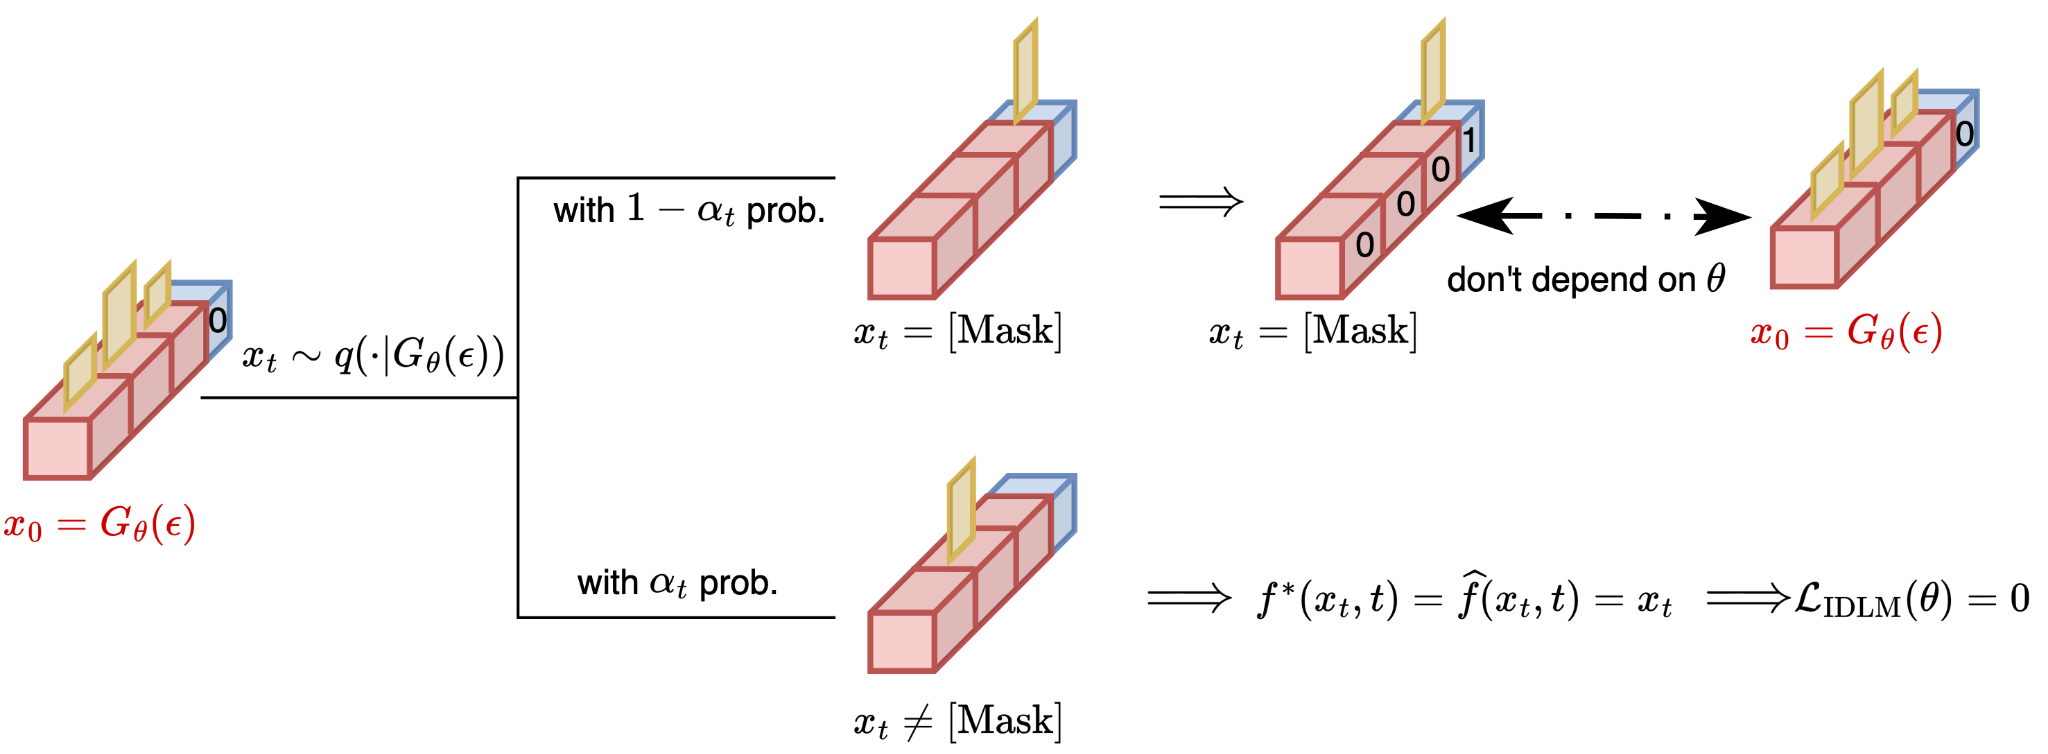
\includegraphics[width=0.95\textwidth]{images/appendix_b_subs_cancellation.png}
    \caption{Mask-only cancellation under \textsc{subs}. The
    masked forward process produces either an unmasked token with probability
    $\alpha_t$ or the mask state with probability $1-\alpha_t$. The unmasked
    branch is copied by \textsc{subs}, so teacher and fake predictions agree and
    its IDLM contribution cancels. The remaining generator signal comes from
    the masked branch.}
    \label{fig:mdlm-subs-cancellation}
\end{figure*}

If $G_\theta(\epsilon)$ denotes the simplex-valued student output used
in the generator update, the MDLM term reduces to the mask-only loss used in
Section~\ref{sec:practical extension of idlm}:
\[
    \LC_{\mathrm{MDLM}}(f,p_\theta)
    =
    -\EE_{\epsilon,t}
    \left[
    (1-\alpha_t)\lambda_t
    \left\langle
    G_\theta(\epsilon),\log f(m,t)
    \right\rangle
    \right].
\]

\paragraph{Teacher-over-fake advantage.}
Consequently, the IDLM-MDLM generator update is driven by the relative
advantage of the teacher over the fake model at the mask state:
\[
    \LC_{\mathrm{IDLM-MDLM}}(\theta)
    =
    -\EE_{\epsilon,t}
    \left[
    (1-\alpha_t)\lambda_t
    \left\langle
    G_\theta(\epsilon),
    \log f^*(m,t)-\log f(m,t)
    \right\rangle
    \right].
\]
This is the mask-only signal used in Section~\ref{sec:practical extension of idlm}.
The sign structure gives the update an attraction--repulsion interpretation.
This is the same teacher-over-fake view developed in
Section~\ref{sec:loss intuition}.
The teacher term attracts the student toward tokens supported by the pretrained
model, while the fake-model term repels tokens that are already easy for a
model trained on the current student samples. Therefore, the student is not
simply pushed toward the teacher's most likely token. A token is promoted when
the teacher assigns it higher log-probability than the fake model does. Once
the fake model catches up with the teacher on student samples, this relative
signal disappears.

\paragraph{Why \textsc{subs} is special.}
The practical benefit is that the generator does not need to backpropagate
through a sampled intermediate token $x_t$. The only generator-dependent object
in the update is the differentiable simplex-valued output $G_\theta(\epsilon)$.
In DMD-like reductions of inverse distillation, an explicit stop-gradient is
usually needed to remove auxiliary gradients through intermediate states
\citep{selikhanovych2025one}. For MDLM, the \textsc{subs} parameterization
effectively handles this cancellation itself: non-mask states are copied and
masked states use the fixed input $m$. In this sense, \textsc{subs} implicitly
applies a stop-gradient to the intermediate state in the generator update. The
resulting mask-only expression resembles the token-level distribution-matching
loss used by discrete MMD distillation~\citep{hoogeboom2026beyond}.
The resemblance is structural rather than exact: D-MMD uses a different
posterior for sampling the intermediate state.
This is a special property of masked diffusion rather than a generic property
of all discrete diffusion processes. In more revisable processes such as
uniform diffusion, gradients through the intermediate state can change the
training behavior substantially; this is tested in Section~\ref{sec:ablation}
and Appendix~\ref{app:ablation-results}.

\paragraph{Beyond \textsc{subs}.}
One can try to pass gradients through masked-diffusion intermediate states
using Gumbel or Argmax relaxations, but this introduces a different problem:
the teacher MDLM is trained on one-hot or mask-token inputs, whereas these
relaxations may feed it simplex-valued states. The resulting teacher signal can
therefore be weaker or less stable. This is why the main IDLM-MDLM update uses
the mask-only \textsc{subs} signal and treats the other relaxations as
ablations in Appendix~\ref{app:ablation-results}.
\end{reviewblock}

\clearpage
\section{\texorpdfstring{\reviewchange{Uniform Diffusion}}{Uniform Diffusion}}
\label{app:uniform process}

\begin{reviewblock}
\reviewchange{This appendix gives the process-specific details for uniform diffusion used by UDLM and Duo in Section~\ref{sec:uniform process duo}, and then explains the corresponding IDLM update from Section~\ref{sec:loss intuition}.}

\subsection{Uniform Diffusion Formulation and Theory}
\label{app:uniform-formulation-theory}
Section~\ref{sec:uniform process duo} introduces uniform diffusion in compact form. Here we unpack the same process: first the CTMC generator and forward kernel, then the UDLM/Duo objective, the Gaussian relaxation used by Duo, and the reverse sampler. This makes explicit which quantities are reused later by the inverse distillation framework in Appendix~\ref{app:uniform-inverse-distillation}.

\paragraph{Forward process.}
Following the general CTMC notation of Appendix~\ref{app:details of considered processes}, the uniform process has terminal distribution $\pi=\frac{1}{N}\vec{1}$. Unlike masked diffusion in Appendix~\ref{app:absorbing process}, which only moves tokens toward the mask, the uniform process lets every token transition to every other token at the same rate. Its base matrix is
\begin{equation}
    Q_{\text{uni}} =
    \begin{bmatrix}
        1 - N & 1 & \cdots & 1 \\
        1 & 1 - N & \cdots & 1 \\
        \vdots & \vdots & \ddots & \vdots \\
        1 & 1 & \cdots & 1 - N
    \end{bmatrix}.
\end{equation}
The time-dependent diffusion matrix is
\begin{equation}
\label{eq: uniform diffusion matrix}
    Q_t = \sigma_t Q_{\text{uni}} =
    \begin{bmatrix}
        \sigma_t(1 - N) & \sigma_t & \cdots & \sigma_t \\
        \sigma_t & \sigma_t(1 - N) & \cdots & \sigma_t \\
        \vdots & \vdots & \ddots & \vdots \\
        \sigma_t & \sigma_t & \cdots & \sigma_t(1 - N)
    \end{bmatrix}.
\end{equation}
Its cumulative transition matrix is
\begin{equation}
    \exp(\bar{\sigma}_t Q_{\text{uni}}) =
    \begin{bmatrix}
        \exp(-N\bar{\sigma}_t) + \frac{1-\exp(-N\bar{\sigma}_t)}{N}
        & \frac{1-\exp(-N\bar{\sigma}_t)}{N} & \cdots & \frac{1-\exp(-N\bar{\sigma}_t)}{N} \\
        \frac{1-\exp(-N\bar{\sigma}_t)}{N}
        & \exp(-N\bar{\sigma}_t) + \frac{1-\exp(-N\bar{\sigma}_t)}{N}
        & \cdots & \frac{1-\exp(-N\bar{\sigma}_t)}{N} \\
        \vdots & \vdots & \ddots & \vdots \\
        \frac{1-\exp(-N\bar{\sigma}_t)}{N}
        & \frac{1-\exp(-N\bar{\sigma}_t)}{N}
        & \cdots & \exp(-N\bar{\sigma}_t) + \frac{1-\exp(-N\bar{\sigma}_t)}{N}
    \end{bmatrix}.
\end{equation}
With $\alpha_t \vcentcolon= \exp(-N\bar{\sigma}_t)$, the conditional distribution used in the main text is therefore
\[
    q_t(x_t\mid x_0)
    = \mathrm{Cat}\bigl(x_t;\alpha_t x_0 + (1-\alpha_t)\tfrac{1}{N}\vec{1}\bigr).
\]
Thus $x_t$ either keeps the clean token or mixes with the uniform distribution; unlike masked diffusion, a trajectory can revise the same position multiple times.

\paragraph{UDLM and Duo objective.}
UDLM~\citep{schiff2024discreteguidance} keeps the clean-token predictor $f(x_t,t)$ but uses the uniform noising law. Duo~\citep{sahoo2025the} uses the same discrete process while evaluating the denoiser on a relaxed input. The main text writes their shared training objective through the compact token-level function $g_{\mathrm{Duo}}$ in Eq.~\eqref{eq:duo loss}. Below we write this function explicitly.

Let $q_t(\cdot\mid x)$ denote the uniform-process transition distribution at time $t$. We use $\tilde{x}_t$ for the input passed to the denoiser and $\bar{x}_t$ for the hard intermediate token whose probability is evaluated in the token-level loss. For UDLM these two objects coincide, $\tilde{x}_t=\bar{x}_t=x_t$. For Duo, $\tilde{x}_t$ is the relaxed model input and $\bar{x}_t$ is the hard token induced by that relaxation. For the corresponding model prediction, write
\[
    f_t\vcentcolon=f(\tilde{x}_t,t).
\]
For the uniform CTMC above, the scalar weight becomes \citep{rutte2025generalized}
\[
    \kappa_t(\bar{x}_t,x_0)
    \vcentcolon=
    \frac{\sigma_t}{q_t(\bar{x}_t\mid x_0)}.
\]
The pointwise Itakura--Saito divergence is
\[
    D_{\mathrm{IS}}(a\|b) \vcentcolon= \frac{a}{b} - \log \frac{a}{b} - 1.
\]
The integrand used in Eq.~\eqref{eq:duo loss} is
\begin{equation}
\label{eq:uniform duo integrand}
g_{\mathrm{Duo}}\bigl(\bar{x}_t,x_0,f_t\bigr)
\vcentcolon=
\lambda_t\kappa_t(\bar{x}_t,x_0)\Bigl[\DC_{\mathrm{KL}}\bigl(q_t(\cdot\mid x_0)\|q_t(\cdot\mid f_t)\bigr) + D_{\mathrm{IS}}\bigl(q_t(\bar{x}_t\mid x_0)\|q_t(\bar{x}_t\mid f_t)\bigr)\Bigr].
\end{equation}
We keep $\lambda_t$ as the optional positive time reweighting used in the main notation. The KL term compares the true and predicted noised distributions. The Itakura--Saito term compares the probability assigned to the currently observed token $\bar{x}_t$, which is the term that later yields the holding-time intuition.

For comparison with the original CTMC notation, the UDLM objective can be written as
\begin{equation}
\label{eq:udlm loss}
\LC_{\mathrm{UDLM}}(f,x_0) = \int_0^1 \EE_{x_t\sim q_t(\cdot\mid x_0)}\bigl[g_{\mathrm{UDLM}}\bigl(x_t,x_0,f(x_t,t)\bigr)\bigr]dt,
\end{equation}
where $g_{\mathrm{UDLM}}$ is the hard-token version of Eq.~\eqref{eq:uniform duo integrand}: set $\tilde{x}_t=\bar{x}_t=x_t$ and $f_t=f(x_t,t)$. Here $q_t(\cdot\mid f_t)$ is obtained by applying the linear forward kernel to the predicted clean-token distribution.

\paragraph{Duo Gaussian relaxation.}
Duo exposes a Gaussian relaxation that makes the noised model input differentiable while keeping the same limiting discrete process. Following the notation of Section~\ref{sec:loss intuition}, introduce an auxiliary Gaussian noise variable and set
\[
    \xi\sim\NC(0,I),
    \qquad
    w_t=\tilde{\alpha}_t x_0+\sqrt{1-\tilde{\alpha}_t^2}\,\xi,
\]
where $\tilde{\alpha}_t$ is the rescaled Duo schedule. The hard intermediate token is obtained by
\[
    \bar{x}_t=x_t(w_t) \vcentcolon= \arg\max(w_t),
    \qquad
    \bar{x}_t\sim q_t(\cdot\mid x_0),
\]
where $\arg\max(w_t)$ denotes the one-hot vector at the largest coordinate. Instead of feeding this hard token to the model, Duo uses the soft approximation
\[
    \tilde{x}_t=x_t^\tau(w_t) = \mathrm{softmax}(w_t/\tau),
\]
which gives the relaxed parameterization $f\colon\Delta\times[0,1]\to\Delta$. With the notation of Eq.~\eqref{eq:duo loss}, Duo evaluates the same KL plus Itakura--Saito divergence objective at $g_{\mathrm{Duo}}(\bar{x}_t,x_0,f(\tilde{x}_t,t))$. As $\tau\to0^+$, the soft input recovers the hard uniform-process token and the objective recovers the UDLM/NELBO limit.

\paragraph{Sampling procedure.}
Sampling starts from the uniform terminal distribution and repeatedly applies reverse transitions estimated from the clean-token predictor. For $0\leq s<t\leq1$, set $\alpha_{t\mid s}\vcentcolon=\alpha_t/\alpha_s$ and $f_t\vcentcolon=f(x_t,t)$. The learned reverse transition used in Section~\ref{sec:uniform process duo} is
\[
p^f_{s\mid t}(x_s\mid x_t)
=
\mathrm{Cat}\!\left(x_s;\frac{N\alpha_t\,x_t\odot f_t+(\alpha_{t\mid s}-\alpha_t)x_t+(\alpha_s-\alpha_t)f_t+(1-\alpha_{t\mid s})(1-\alpha_s)\vec{1}/N}{N\alpha_t\langle x_t,f_t\rangle+1-\alpha_t}\right).
\]
This reverse step can either keep the current token or move to another token, so the sampler has a timing decision in addition to a token-choice decision, as illustrated in Figure~\ref{fig:appendix process intuition}. This is the main structural difference from masked diffusion.

\subsection{Inverse Distillation for Uniform Diffusion}
\label{app:uniform-inverse-distillation}
We now connect the uniform diffusion process to the IDLM objective. The ideal
inverse-distillation loss compares the pretrained teacher $f^*$ with the best
diffusion model that could be trained only on the current student distribution:
\begin{equation}
\label{eq:idlm-duo-compact}
    \LC_{\mathrm{IDLM\text{-}Duo}}(\theta)
    \vcentcolon=
    \LC_{\mathrm{Duo}}(f^*,p_\theta)
    -
    \min_{\tilde f}\LC_{\mathrm{Duo}}(\tilde f,p_\theta).
\end{equation}
In practice, as in Section~\ref{sec:loss intuition}, we alternate between
training the fake model and updating the generator. During the generator step,
the fake model $f$ is fixed. Write
\[
    f_t^* \vcentcolon= f^*(\tilde{x}_t,t),
    \qquad
    f_t \vcentcolon= f(\tilde{x}_t,t)
\]
for the teacher and fake predictions at the Duo input. The objective becomes
\begin{equation}
\label{eq:idlm-duo-fixed}
\begin{aligned}
    \LC_{\mathrm{IDLM\text{-}Duo}}(\theta)
    &\vcentcolon=
    \LC_{\mathrm{Duo}}(f^*,p_\theta)
    -
    \LC_{\mathrm{Duo}}(f,p_\theta)
    \\
    &=
    \EE_{\epsilon,t,\xi}
    \Bigl[
    \lambda_t\kappa_t(\bar{x}_t,G_\theta(\epsilon))
    \Bigl(
    \\
    &\quad
    \sum_{y\in\VC}q_t(y\mid G_\theta(\epsilon))\log\frac{q_t(y\mid f_t)}{q_t(y\mid f_t^*)}
    + q_t(\bar{x}_t\mid G_\theta(\epsilon))
    \left(\frac{1}{q_t(\bar{x}_t\mid f_t^*)}-\frac{1}{q_t(\bar{x}_t\mid f_t)}\right)
    + \log\frac{q_t(\bar{x}_t\mid f_t^*)}{q_t(\bar{x}_t\mid f_t)}
    \Bigr)
    \Bigr].
\end{aligned}
\end{equation}
Here $G_\theta(\epsilon)$ is the relaxed student sample, and
$(\bar{x}_t,\tilde{x}_t)$ are the hard and relaxed Duo states defined below.
This is the same teacher-minus-fake principle as in Appendix~\ref{app:mdlm-inverse-distillation}, but the uniform process does not collapse to a mask-only term.

\paragraph{Simplex relaxation.}
We use the same simplex relaxation as in Section~\ref{sec:simplex relaxation}
and Appendix~\ref{app:mdlm-inverse-distillation}. The generator output is
allowed to be a token distribution,
\[
    G_\theta(\epsilon)\in\Delta ,
\]
which is the same relaxation illustrated in
Figure~\ref{fig:mdlm-simplex-relaxation}. The uniform forward kernel is linear
in the clean token, so it remains well-defined on this relaxed output:
\[
    q_t(\cdot\mid G_\theta(\epsilon))
    =
    \alpha_tG_\theta(\epsilon)+(1-\alpha_t)\tfrac{1}{N}\vec{1}
    \in\Delta .
\]
Thus, as in the masked case, the generator can receive gradients through
weighted token probabilities instead of through a hard one-hot choice.

\paragraph{Gaussian reparameterization.}
The second issue is the intermediate uniform token. Unlike masked diffusion,
uniform diffusion can move from any token to any other token, so the sampled
intermediate state cannot be removed by the \textsc{subs} cancellation. Duo
resolves this by sampling a Gaussian latent variable whose noise is independent
of the generator output:
\[
    \xi\sim\NC(0,I),
    \qquad
    w_t=\tilde{\alpha}_tG_\theta(\epsilon)
    +\sqrt{1-\tilde{\alpha}_t^2}\,\xi .
\]
The hard token used in the token-level loss and the relaxed input passed to
the denoiser are
\[
    \bar{x}_t=\arg\max(w_t),
    \qquad
    \tilde{x}_t=\mathrm{softmax}(w_t/\tau).
\]
Equivalently, the full differentiable transition from the generator output to
the relaxed Duo input is
\[
    G_\theta(\epsilon)
    \mapsto
    \tilde{x}_t
    =
    \mathrm{softmax}\!\left(
    \frac{\tilde{\alpha}_tG_\theta(\epsilon)
    +\sqrt{1-\tilde{\alpha}_t^2}\,\xi}{\tau}
    \right),
    \qquad
    \xi\sim\NC(0,I).
\]
These definitions make the fixed-fake objective in Eq.~\eqref{eq:idlm-duo-fixed}
fully reparameterized and keep the intermediate-state path differentiable.

\paragraph{Teacher-over-fake advantage.}
Following the local-advantage notation of Section~\ref{sec:loss intuition}, define
\[
a_t \vcentcolon= g_{\mathrm{Duo}}(\bar{x}_t,G_\theta(\epsilon),f_t^*) - g_{\mathrm{Duo}}(\bar{x}_t,G_\theta(\epsilon),f_t).
\]
Using Eq.~\eqref{eq:uniform duo integrand}, and dropping the common positive
weight $\lambda_t\kappa_t(\bar{x}_t,G_\theta(\epsilon))$, the local advantage
expands to
\[
\begin{aligned}
\bigl(\lambda_t\kappa_t(\bar{x}_t,G_\theta(\epsilon))\bigr)^{-1}a_t
&=
-\left\langle q_t(\cdot\mid G_\theta(\epsilon)),\log\frac{q_t(\cdot\mid f_t^*)}{q_t(\cdot\mid f_t)}\right\rangle
\\
&\quad
+ q_t(\bar{x}_t\mid G_\theta(\epsilon))
\left(\frac{1}{q_t(\bar{x}_t\mid f_t^*)}-\frac{1}{q_t(\bar{x}_t\mid f_t)}\right)
+ \log\frac{q_t(\bar{x}_t\mid f_t^*)}{q_t(\bar{x}_t\mid f_t)}.
\end{aligned}
\]
The first term is the distribution-level teacher-over-fake signal at time $t$.
The remaining terms compare how much probability the teacher and fake model
assign to the current intermediate token $\bar{x}_t$.

\paragraph{Intuition.}
Uniform diffusion can revise the same position more than once. At each reverse
step, the sampler decides whether to keep the current token or replace it.
The first term in the local advantage is the time-$t$ analogue of the
distribution-level attraction--repulsion signal from masked diffusion
(Appendix~\ref{app:mdlm-inverse-distillation}):
\begingroup\small
\[
-\left\langle q_t(\cdot\mid G_\theta(\epsilon)),
\log\frac{q_t(\cdot\mid f_t^*)}{q_t(\cdot\mid f_t)}\right\rangle
=
\DC_{\mathrm{KL}}\!\left(q_t(\cdot\mid G_\theta(\epsilon))\|q_t(\cdot\mid f_t^*)\right)
-
\DC_{\mathrm{KL}}\!\left(q_t(\cdot\mid G_\theta(\epsilon))\|q_t(\cdot\mid f_t)\right).
\]
\endgroup
Thus, it favors generator samples whose distribution after uniform noising at
time $t$ is closer to the teacher than to the fake model. Compared with masked
diffusion, this comparison is not made directly on clean-token distributions:
the uniform CTMC first mixes each token toward the uniform stationary
distribution, and the amount of mixing depends on $t$. The signal is therefore
a difference between KL divergences of the time-dependent noised distributions.
The holding-time intuition is controlled by the probability assigned to the
current intermediate token: larger $q_t(\bar{x}_t\mid f_t^*)$ corresponds to a
longer teacher holding time at $\bar{x}_t$, while smaller
$q_t(\bar{x}_t\mid f_t^*)$ corresponds to a shorter one. This effect appears
directly in the current-token part of Eq.~\eqref{eq:idlm-duo-fixed}:
\[
q_t(\bar{x}_t\mid G_\theta(\epsilon))
\left(
\frac{1}{q_t(\bar{x}_t\mid f_t^*)}
-
\frac{1}{q_t(\bar{x}_t\mid f_t)}
\right)
+
\log\frac{q_t(\bar{x}_t\mid f_t^*)}{q_t(\bar{x}_t\mid f_t)}.
\]
For a fixed intermediate token, the coefficient of
$q_t(\bar{x}_t\mid G_\theta(\epsilon))$ is
\[
c_t(\bar{x}_t)
\vcentcolon=
\frac{1}{q_t(\bar{x}_t\mid f_t^*)}
-
\frac{1}{q_t(\bar{x}_t\mid f_t)}.
\]
If $q_t(\bar{x}_t\mid f_t^*)$ is small, then $c_t(\bar{x}_t)$ is large and
positive, so minimizing the loss pushes the generator to reduce the probability
of clean samples whose noising lands at $\bar{x}_t$. This agrees with the
holding-time view: the teacher reverse process has a large exit rate at such an
intermediate state and would leave it quickly, so the generator is discouraged
from producing samples whose uniform noising often visits that state. If the
teacher probability is large while the fake-model probability is small, then
$c_t(\bar{x}_t)<0$. Since it minimizes the IDLM loss, the generator is pushed
toward clean samples whose uniform noising visits such teacher-supported states
more often; the small fake-model probability strengthens this preference through
the negative term $-1/q_t(\bar{x}_t\mid f_t)$. This is the uniform-process
analogue of the attraction--repulsion interpretation in
Appendix~\ref{app:mdlm-inverse-distillation}: teacher-supported states attract
the generator, while the fake model's low probability makes this signal
stronger. In the next alternating step, the fake model is trained on the updated generator
distribution, so it adapts to these states and reduces the teacher--fake gap
there. Thus, the uniform loss teaches both which token should be chosen and how
long the sampler should stay in the current intermediate state.

\paragraph{DMD-like stop-gradient for uniform diffusion.}
The ablation in Section~\ref{sec:ablation} and
Appendix~\ref{app:ablation-results} compares the full IDLM-Duo update with a
stop-gradient variant. In the idealized objective, IDLM matches complete diffusion path
measures,
\[
    \LC_{\mathrm{IDLM}}(\theta)
    =
    \DC_{\mathrm{KL}}(\PP^\theta\|\PP^*),
\]
where $\PP^\theta$ and $\PP^*$ are the path measures induced by the student and
data distributions. For any time $t$, let
\[
    p_t^\theta(x_t)=\int q_t(x_t\mid x_0)\,p_\theta(dx_0),
    \qquad
    p_t^*(x_t)=\int q_t(x_t\mid x_0)\,p^*(dx_0).
\]
A DMD-like reduction, as shown by RSD~\citep{selikhanovych2025one}, replaces
the path-measure objective by noised-marginal matching,
\[
    \LC_{\mathrm{DMD\text{-}like}}(\theta)
    =
    \EE_t\!\left[
    \DC_{\mathrm{KL}}(p_t^\theta\|p_t^*)
    \right],
\]
and treats the intermediate state as fixed in the generator update. In the Duo
parameterization this corresponds to replacing the full relaxed path
\[
    w_t
    =
    \tilde{\alpha}_tG_\theta(\epsilon)
    +\sqrt{1-\tilde{\alpha}_t^2}\,\xi
\]
by its stop-gradient version
\[
    w_t^{\mathrm{sg}}
    =
    \tilde{\alpha}_t\mathrm{sg}\!\left(G_\theta(\epsilon)\right)
    +\sqrt{1-\tilde{\alpha}_t^2}\,\xi .
\]
Thus, the DMD-like stop-gradient objective optimizes a marginal matching problem
rather than the path-level IDLM-Duo objective. Empirically, this distinction is
important: Figure~\ref{fig:ablation-uniform} shows that IDLM-Duo with stop-gradient
quickly enters a high-entropy, high-GenPPL regime, while the full IDLM-Duo update
remains stable.

\begin{figure}[t]
    \centering
    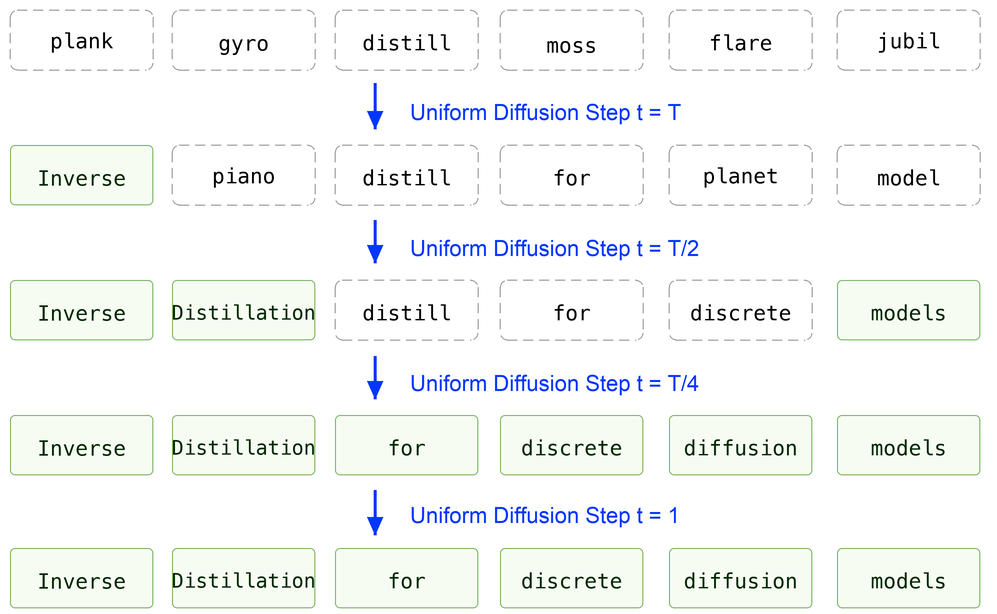
\includegraphics[width=\textwidth]{images/uniform_diffusion_assembly.png}
    \caption{Uniform diffusion sampling. Unlike masked diffusion, a position can be revised multiple times, so each step must decide both whether to hold or change the current token and which token should replace it.}
    \label{fig:appendix process intuition}
\end{figure}
\end{reviewblock}
